This Generalized Van Der Pol oscillator was proposal by Schurz in \cite{Schurz2003}:\\
Schurz, H. General Theorems for Numerical Approximations of Stochastic Processes on the Hilbert 
Space $H_2([0,T], \mu, \mathbb{R}^d)$
\begin{align}
	dX_t^{(1)}	&= X_t^{(2)} dt\\
	dX_t^{(2)}&=
	\left[
		-\omega^2 X_t^{(1)} 
		+\sigma 
		\left(
			1 - \mu_1 \left( X_t^{(1)} \right)^2
			-\mu_2 \left( X_t \right)^2
		\right)
			X_t^{(2)}
	\right]dt
	+\sigma X_t^{(2)} dW_t \label{eqn:GeneralizedVanDerPol1}.
\end{align}
Right now we had constructed the following Linearized Steklov Scheme:
\begin{align}
	a_1^{(2)}(x,y)&:= \gamma (1-\mu_1 x^2 - \mu_2 y^2 ), \qquad
	a_2^{(2)}(x):= -\omega^2 x, \notag \\
	X_{k+1}^{(1)}&=	X_k^{(1)} + h X_k^{(2)}, \\
	X_{k+1}^{(2)}&= 
		\left(
			X_{k}^{(2)}
			+
			\frac{
					a_2
					\left(
						X_{k+1}^{(1)}
					\right)
			}
			{
				a_1^{(2)}
				\left(
					X_{k+1}^{(1)}, X_k^{(2)}
				\right)
			}
		\right)
		\exp
		\left(
			a_1^{(2)}
			\left(
				X_{k+1}^{(1)}, X_k^{(2)}
			\right) h
		\right)
		+\sigma  X_{k}^{(2)} \Delta W_k.
	\notag
\end{align}
This scheme follows almost the same profile of numerical solutions of the Partial Linear
Implicit proposal by Schurz.
\begin{figure}[htb]
\centering
	% GNUPLOT: LaTeX picture with Postscript
\begingroup
  \fontfamily{Times-New-Roman}%
  \selectfont
  \makeatletter
  \providecommand\color[2][]{%
    \GenericError{(gnuplot) \space\space\space\@spaces}{%
      Package color not loaded in conjunction with
      terminal option `colourtext'%
    }{See the gnuplot documentation for explanation.%
    }{Either use 'blacktext' in gnuplot or load the package
      color.sty in LaTeX.}%
    \renewcommand\color[2][]{}%
  }%
  \providecommand\includegraphics[2][]{%
    \GenericError{(gnuplot) \space\space\space\@spaces}{%
      Package graphicx or graphics not loaded%
    }{See the gnuplot documentation for explanation.%
    }{The gnuplot epslatex terminal needs graphicx.sty or graphics.sty.}%
    \renewcommand\includegraphics[2][]{}%
  }%
  \providecommand\rotatebox[2]{#2}%
  \@ifundefined{ifGPcolor}{%
    \newif\ifGPcolor
    \GPcolorfalse
  }{}%
  \@ifundefined{ifGPblacktext}{%
    \newif\ifGPblacktext
    \GPblacktexttrue
  }{}%
  % define a \g@addto@macro without @ in the name:
  \let\gplgaddtomacro\g@addto@macro
  % define empty templates for all commands taking text:
  \gdef\gplbacktext{}%
  \gdef\gplfronttext{}%
  \makeatother
  \ifGPblacktext
    % no textcolor at all
    \def\colorrgb#1{}%
    \def\colorgray#1{}%
  \else
    % gray or color?
    \ifGPcolor
      \def\colorrgb#1{\color[rgb]{#1}}%
      \def\colorgray#1{\color[gray]{#1}}%
      \expandafter\def\csname LTw\endcsname{\color{white}}%
      \expandafter\def\csname LTb\endcsname{\color{black}}%
      \expandafter\def\csname LTa\endcsname{\color{black}}%
      \expandafter\def\csname LT0\endcsname{\color[rgb]{1,0,0}}%
      \expandafter\def\csname LT1\endcsname{\color[rgb]{0,1,0}}%
      \expandafter\def\csname LT2\endcsname{\color[rgb]{0,0,1}}%
      \expandafter\def\csname LT3\endcsname{\color[rgb]{1,0,1}}%
      \expandafter\def\csname LT4\endcsname{\color[rgb]{0,1,1}}%
      \expandafter\def\csname LT5\endcsname{\color[rgb]{1,1,0}}%
      \expandafter\def\csname LT6\endcsname{\color[rgb]{0,0,0}}%
      \expandafter\def\csname LT7\endcsname{\color[rgb]{1,0.3,0}}%
      \expandafter\def\csname LT8\endcsname{\color[rgb]{0.5,0.5,0.5}}%
    \else
      % gray
      \def\colorrgb#1{\color{black}}%
      \def\colorgray#1{\color[gray]{#1}}%
      \expandafter\def\csname LTw\endcsname{\color{white}}%
      \expandafter\def\csname LTb\endcsname{\color{black}}%
      \expandafter\def\csname LTa\endcsname{\color{black}}%
      \expandafter\def\csname LT0\endcsname{\color{black}}%
      \expandafter\def\csname LT1\endcsname{\color{black}}%
      \expandafter\def\csname LT2\endcsname{\color{black}}%
      \expandafter\def\csname LT3\endcsname{\color{black}}%
      \expandafter\def\csname LT4\endcsname{\color{black}}%
      \expandafter\def\csname LT5\endcsname{\color{black}}%
      \expandafter\def\csname LT6\endcsname{\color{black}}%
      \expandafter\def\csname LT7\endcsname{\color{black}}%
      \expandafter\def\csname LT8\endcsname{\color{black}}%
    \fi
  \fi
  \setlength{\unitlength}{0.0500bp}%
  \begin{picture}(7936.00,4902.00)%
    \gplgaddtomacro\gplbacktext{%
      \colorrgb{0.50,0.50,0.50}%
      \put(620,703){\makebox(0,0)[r]{\strut{}-8}}%
      \colorrgb{0.50,0.50,0.50}%
      \put(620,1395){\makebox(0,0)[r]{\strut{}-6}}%
      \colorrgb{0.50,0.50,0.50}%
      \put(620,2087){\makebox(0,0)[r]{\strut{}-4}}%
      \colorrgb{0.50,0.50,0.50}%
      \put(620,2779){\makebox(0,0)[r]{\strut{}-2}}%
      \colorrgb{0.50,0.50,0.50}%
      \put(620,3470){\makebox(0,0)[r]{\strut{} 0}}%
      \colorrgb{0.50,0.50,0.50}%
      \put(620,4162){\makebox(0,0)[r]{\strut{} 2}}%
      \colorrgb{0.50,0.50,0.50}%
      \put(620,4854){\makebox(0,0)[r]{\strut{} 4}}%
      \colorrgb{0.50,0.50,0.50}%
      \put(803,440){\makebox(0,0){\strut{}-1}}%
      \colorrgb{0.50,0.50,0.50}%
      \put(1555,440){\makebox(0,0){\strut{}-0.5}}%
      \colorrgb{0.50,0.50,0.50}%
      \put(2308,440){\makebox(0,0){\strut{} 0}}%
      \colorrgb{0.50,0.50,0.50}%
      \put(3060,440){\makebox(0,0){\strut{} 0.5}}%
      \colorrgb{0.50,0.50,0.50}%
      \put(3813,440){\makebox(0,0){\strut{} 1}}%
      \colorrgb{0.50,0.50,0.50}%
      \put(4565,440){\makebox(0,0){\strut{} 1.5}}%
      \colorrgb{0.50,0.50,0.50}%
      \put(5318,440){\makebox(0,0){\strut{} 2}}%
      \colorrgb{0.50,0.50,0.50}%
      \put(6070,440){\makebox(0,0){\strut{} 2.5}}%
      \colorrgb{0.50,0.50,0.50}%
      \put(6823,440){\makebox(0,0){\strut{} 3}}%
      \colorrgb{0.50,0.50,0.50}%
      \put(7575,440){\makebox(0,0){\strut{} 3.5}}%
      \csname LTb\endcsname%
      \put(160,2778){\rotatebox{-270}{\makebox(0,0){\strut{}$X^{(2)}_k$}}}%
      \put(4189,140){\makebox(0,0){\strut{}$X^{(1)}_k$}}%
    }%
    \gplgaddtomacro\gplfronttext{%
      \csname LTb\endcsname%
      \put(6672,4691){\makebox(0,0)[r]{\strut{}Exact}}%
      \csname LTb\endcsname%
      \put(6672,4491){\makebox(0,0)[r]{\strut{}SSLS h =.001}}%
      \csname LTb\endcsname%
      \put(6672,4291){\makebox(0,0)[r]{\strut{}PLIE h =.001}}%
    }%
    \gplbacktext
    \put(0,0){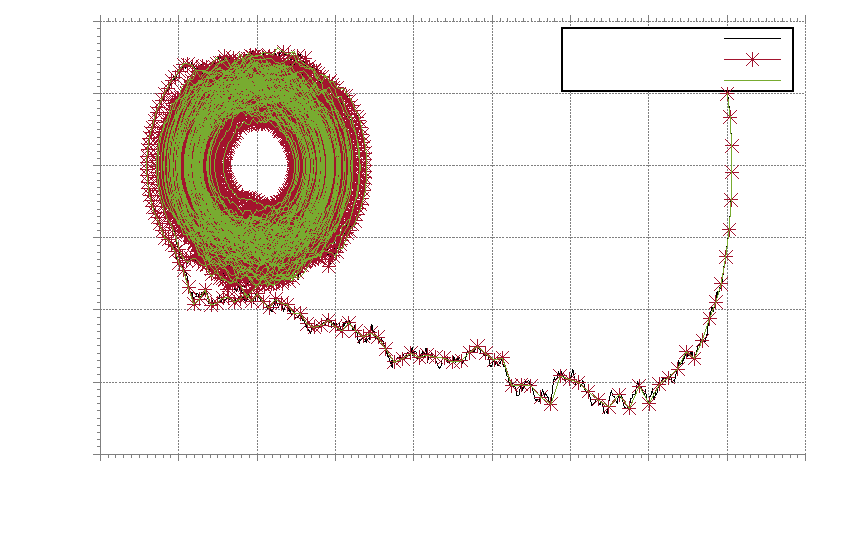
\includegraphics{./papers/paperB/figures/PhasePotrait}}%
    \gplfronttext
  \end{picture}%
\endgroup

	\caption{'Typical' trajectory of SDE \eqref{eqn:GeneralizedVanDerPol1}
		with 
		$\omega = \num{5}$, 
		$\gamma = \num{1.0}$,
		$\mu_1 = \num{0.05}$,
		$\mu_2 = \num{0.25}$,
		$\sigma = \num{0.5}$,
		$X_0 = (\num{3}, \num{2})^T$
		and discretized with the SSLS and PLIE schemes. Here exact means a discretization with the EM 
		scheme using a step size of $h=\num{1e-4}$.
	}
\label{fig:GenVanDerPolPhasePotrait}
\end{figure}



















































